\section{Appendix: Derivations}

\subsection{Derivation of conditional block distribution given feature matrix}
\label{appdx:b|x}

We wish to determine the form of $p(b| X)$. This can be done by integrating over the joint probability with respect to $\theta$.
%
\begin{align*}
	p(b | X) &= \int p(b , \theta| X, \theta) d\theta = \int p(b | X, \theta) p(\theta | X) d\theta \\
	&=\int p(b | X, \theta) p(\theta) d\theta = \int \prod_{i \in [N] } \phi_{b_i}(x_i; \theta) p(\theta) d\theta \\
	&= \prod_{i \in [N]} \int \frac{\exp(w_{b_i}^T \tilde{x}_i) \prod_{j \in [B]} \Gaussian(w_j; 0, \sigma_\theta^2 I)}{\sum_{k \in [B]} \exp(w_{k}^T \tilde{x}_i)} dw_{1:B}
\end{align*}
%
We note that $b_i \in [B]$ and so the integral's value is unchanged with respect to $b_i$. The integrand has the same form no matter which value $b_i$ takes as the prior is the same for each $w_j$. As such the integral can only be a function of at most $\tilde{x}_i$ and $\sigma_\theta^2$ as it is symmetric with respect to $b_i$ and all the various $w_j$ are integrated out as they are dummy variables. Therefore, denoting the integral by the (unknown) function $f(\tilde{x}_i, \sigma_\theta^2)$, we write $p(b| X)$ as follows:
%
\begin{align*}
	p(b | X) &= \prod_{i=1}^{N} f(\tilde{x}_i, \sigma_\theta^2) = \textrm{const w.r.t } b = c
\end{align*}
%
As this is a constant with respect to $b$ we conclude that $p(b | X)$ must be a uniform distribution. $\nicefrac{1}{c}$ is simply the size of the set of values that $b$ can take. We know $b_i \in [B]$. Therefore, $b \in [B]^N$ and $|[B]^N| = B^N = \nicefrac{1}{c}$. Putting this all together we conclude that:
%
\begin{equation}
	p(b | X) = B^{-N}
\end{equation}

\subsection{Derivation of U form}
\label{appdx:form-U}

The invariant distribution we wish to target for the $\theta$ samples is the posterior of $\theta$ given the values of the pair $(X, b)$. We write this as follows:
%
\begin{align}
	\pi_\theta(\theta) &\propto p(\theta | X, b) \propto p(b | X, \theta) p(\theta) \propto  \exp \left( - U(\theta) \right) \\
	\therefore U(\theta) &= - \left( \log p(b | X, \theta) + \log p(\theta) \right) + \textrm{const}
\end{align}
%
Where we have introduced $U(\theta)$ equal to the negative log posterior. Each of the constituent terms of $U(\theta)$ are easily computed (equation \ref{eqn:U-constituent-terms}) by defining $y_{ij} \coloneqq \one \left\{ b_i = j \right\}$ and $a_{ij} \coloneqq \phi_j(x_i; \theta)$.
%
\begin{equation}
	\log p(b | X, \theta) = \sum_{i \in [N]} \sum_{j \in [B]} y_{ij} \log a_{ij}  \quad \textrm{and} \quad
	\log p(\theta) = -\frac{(D+1)(B)}{2} \log 2\pi - \frac{1}{2 \sigma_\theta^2} || \theta ||^2
	\label{eqn:U-constituent-terms}
\end{equation}
%
Discarding constant terms, we write $U(\theta)$ as in equation \ref{eqn:U-form-appdx-0}. Note that $||\theta||^2 = \sum_{i} \theta_{i}^2 = \sum_{j=1}^{B} ||w_j||^2$ is the Euclidean norm of the vector of parameters $\theta$.
%
\begin{equation}
	U(\theta) = \left( \sum_{i=1}^{N} \sum_{j=1}^{B} y_{ij} \log \frac{1}{a_{ij}} \right)
	+ \frac{1}{2\sigma_\theta^2} ||\theta||^2 = N \cdot \Lcal(\theta) + \frac{1}{2\sigma_\theta^2} ||\theta||^2
	\label{eqn:U-form-appdx-0}
\end{equation}
%

\subsection{Derivation of U gradient with respect to feature parameters}
\label{appdx:gradu}
The goal is to determine $\nabla U(\theta)$, the gradient of the negative log posterior with respect to the parameters. We repeat the form of $U(\theta)$ in equation \ref{eqn:U-form-appdx}.
%
\begin{equation}
	U(\theta) = \left( \sum_{i \in [N]} \sum_{j \in [B]} y_{ij} \log \frac{1}{a_{ij}} \right)
	+ \frac{1}{2\sigma_\theta^2} ||\theta||^2
	\label{eqn:U-form-appdx}
\end{equation}
%
Where $y_{ij}$ is independent of $\theta$ and $a_{ij}$ is the output from the softmax layer, with form as given in equation \ref{eqn:a-ij}.
%
\begin{equation}
	a_{ij} \coloneqq \phi_{j} (x_i; \theta) = \frac{\exp(w_j^T \tilde{x}_i)}{\sum_{r \in [B]} \exp(w_r^T \tilde{x}_i)}
	\label{eqn:a-ij} 
\end{equation}
%
We note that $\theta = \{w_k\}_{k=1}^B$, and as such we can write this in vector form $\theta = \left[w_1^T, w_2^T \dots w_B^T  \right]^T$. Therefore, $\nabla U(\theta) = \left[\nicefrac{\partial U}{\partial w_1}^T,\nicefrac{\partial U}{\partial w_2}^T \dots \nicefrac{\partial U}{\partial w_B}^T  \right]^T$; to compute $\nabla U(\theta)$ it suffices to find the form of $\nicefrac{\partial U}{\partial w_k}$ with respect to a general $k$.

To this end, we must first find partial derivatives of $a_{ij}$ and $||\theta||$ with respect to $w_k$. Starting with $a_{ij}$:
%
\begin{align}
	\frac{\partial a_{ij}}{\partial w_k} &= \frac
	{\tilde{x}_i \exp(w_j^T \tilde{x}_i) \delta_{jk} \cdot \sum_{r \in [B]} \exp(w_r^T \tilde{x}_i) 
		- 
		\exp(w_j^T \tilde{x}_i) \cdot \tilde{x}_i \exp(w_k^T \tilde{x}_i)}
	{\left( \sum_{r \in [B]} \exp(w_r^T \tilde{x}_i) \right)^2} \nonumber \\
	&= \tilde{x}_i \left( a_{ij} \delta_{jk} - a_{ij}a_{ik} \right) 
\end{align}
%
Where $\delta_{jk} \coloneqq \one \left\{ j = k \right\}$. Now moving onto the derivative of $||\theta||^2$:
%
\begin{equation}
	\frac{ \partial}{\partial w_k} ||\theta||^2 = \frac{\partial}{\partial w_k} \left( \sum_{r \in [B]} ||w_r||^2 \right) = 2w_k
\end{equation}
%
We are ready to put this all together, to find the partial derivative of $U(\theta)$ with respect to each $w_k$:
\begin{align}
	\frac{\partial U}{\partial w_k} &= 
	\sum_{i=1}^{N} \sum_{j=1}^{B} y_{ij} 
	\left( \frac{-\tilde{x}_i}{a_{ij}} \left( a_{ij} \delta_{jk} - a_{ij} a_{ik} \right) \right)
	+ \frac{w_k}{\sigma_\theta^2} \nonumber \\
	&=  - \left( \sum_{i=1}^{N} \tilde{x}_i \left( y_{ik} - a_{ik} \sum_{j=1}^{B} y_{ij} \right)
	- \frac{w_k}{\sigma_\theta^2} \right) \nonumber \\
	&= - \left( \sum_{i=1}^{N} \Big\{ \tilde{x}_i (y_{ik} - a_{ik}) \Big\} - \frac{w_k}{\sigma_\theta^2} \right)
\end{align}
%
This is the required result. This form can be computed efficiently through matrix operations. The only property of $y_{ij}$ we have used in the derivation is the sum-to-one constraint $\sum_{j=1}^{B} y_{ij} = 1$ for all $i$.

\subsection{Hypothesis test on feature weights}

We are given samples $\{\theta^{(t)}\}_{t \in \Tcal_\theta} \sim p(\theta | A, X)$ and wish to determine the statistical significance of the weights. We adopt matrix notation for simplicity by representing $\theta$ with the matrix $B \times D$ matrix of feature weights $W$. The question is to determine the significance of a particular feature $d$ by examining the value of $W_{id}$ for all the values $i \in [B]$. We know that the posterior is proportional to the prior multiplied by the likelihood (assuming that the feature matrix $X$ is already given):
%
\begin{equation}
	p(\theta|A, X) \propto p(\theta) \cdot p(A | \theta, X)
\end{equation}
%
The prior term can be evaluated but the likelihood is intractable. The closest we can get is through a Monte-Carlo integration over $b$:
%
\begin{align}
	p(A | \theta, X) &= \sum_{b \in [B]^N} p(A, b | \theta, X) \nonumber \\
	&= \sum_{b \in [B]^N} p(A | b, \theta, X) \cdot p(b | \theta, X) \nonumber \\
	&= \sum_{b \in [B]^N} p(A | b) \cdot p(b | \theta, X) \nonumber \\
	&\approx \sum_{i} p\left( A | b^{(i)} \right) \quad \textrm{with} \quad b^{(i)} \sim p(b| \theta, X)
	\label{eqn:mc-likelihood}
\end{align}
%
This could be implemented for a single value of $\theta$ but such a form cannot be used to characterise the overall form of the posterior. Nevertheless, the form in equation \ref{eqn:mc-likelihood} still does highlight something interesting. The likelihood is peaked around areas of $\theta$ that generate a partition $b$ that is highly likely in the SBM sense -- high $p(A|b)$. This provides the motivation for using the Laplace approximation for modelling the posterior $p(\theta | A, X) \approx p(\theta; \mu, \Sigma)$. Indeed, the Laplace approximation is often used for modelling the posterior in logistic classification \cite{laplace}. As a simplification we assume that $\Sigma$ is diagonal, therefore each element of $\theta$ is independent. This assumption does not hold in general but it motivates the derivation of the dimensionality reduction we construct by analogy with hypothesis testing. Assuming, $\Sigma$ is diagonal then the posterior for each element of the weight matrix $W$ can be approximated by:
%
\begin{equation}
	p(W_{ij}|A, X) \approx \Gaussian(W_{ij}|\hat{\mu}_{ij}, \hat{\sigma}_{ij}^2)
\end{equation}
%
Where we have used the set of samples for $W$ drawn according to the exact posterior, to calculate unbiased estimates for the mean and standard deviation:
%
\begin{equation}
	\hat{\mu}_{ij} \coloneqq \frac{1}{|\Tcal_\theta|} \sum_{t \in \Tcal_\theta} W_{ij}^{(t)} \qquad \textrm{and} \qquad
	\hat{\sigma}_{ij}^2 \coloneqq \frac{1}{|\Tcal_\theta|} \sum_{t \in \Tcal_\theta} \left( W_{ij}^{(t)} - \hat{\mu}_{ij} \right)^2
\end{equation}
%
This approximation is not exact but can show it is accurate empirically. Indeed, if we run the primary school experiment with hyper-parameters given in appendix \ref{appdx:hyperparams}, we can then plot histograms of the collected $W$-samples and compare these to the Laplace approximation. The results are given on figure \ref{fig:school-histogram}. Even though the Laplace approximation is not exact, it is remarkably reliable. 

\begin{figure}[!h]
	\centering
	\begin{subfigure}[t]{0.3\linewidth}
		\centering
		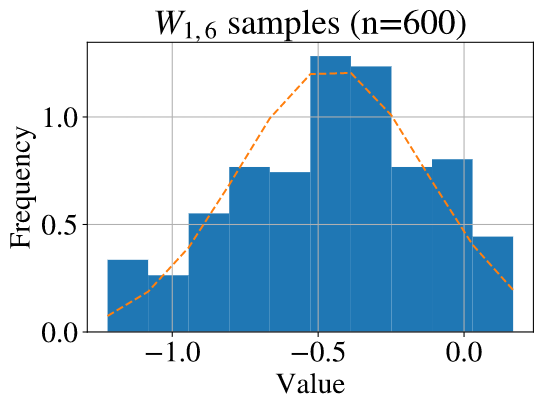
\includegraphics[width=\linewidth]{school-sample-histogram-16.png}
		\caption{Weight for block 1, class 3B}
	\end{subfigure}
	\hfill
	\begin{subfigure}[t]{0.3\linewidth}
		\centering
		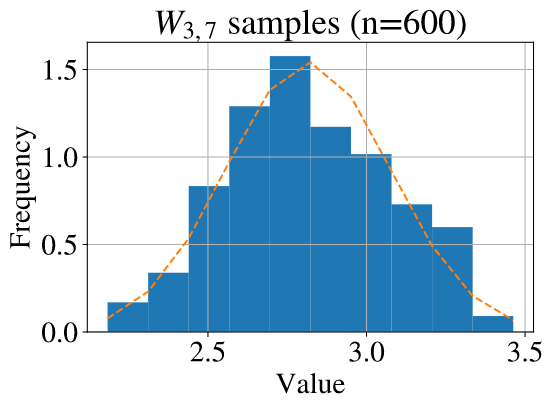
\includegraphics[width=\linewidth]{school-sample-histogram-37.png}
		\caption{Weight for block 3, class 4A}
	\end{subfigure}
	\hfill
	\begin{subfigure}[t]{0.3\linewidth}
		\centering
		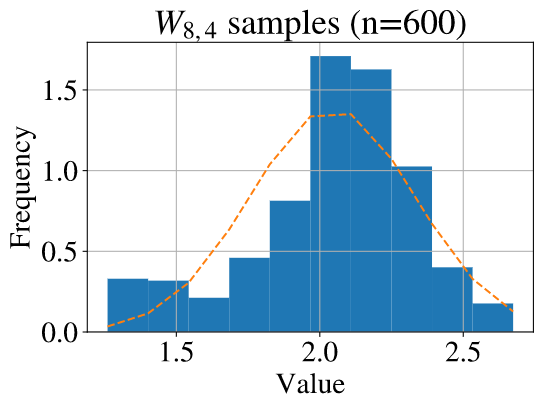
\includegraphics[width=\linewidth]{school-sample-histogram-84.png}
		\caption{Weight for block 8, class 2B}
	\end{subfigure}

	\caption{Histograms of sampled weights for the primary school experiment \cite{schools}. Dotted line is the applied Laplace approximation.}
	\label{fig:school-histogram}
\end{figure}

Using the approximation, we can construct a test to determine whether a particular weight value has $|W_{ij}| > c$ with high probability. Assuming without loss of generality that
%
\begin{equation}
	p(|W_{ij}| > c) = p(W_{ij})
\end{equation}